\chapter{Конструкторская часть}

В данном разделе представлены схемы алгоритма полного перебора и муравьиного алгоритма.

\section{Разработка алгоритма полного перебора}
На рис. \ref{img:schema1} представлена схема алгоритма полного перебора.

\begin{figure}[h!]
\centering
    \includegraphics[width=0.9\linewidth]{schema1.pdf}
    \caption{Схема алгоритма полного перебора}
    \label{img:schema1}	
\end{figure}

\section{Разработка муравьиного алгоритма}
На рис. \ref{img:schema2}~--~\ref{img:schema4} представлена схема муравьиного алгоритма.

\newpage

\begin{figure}[h!]
\centering
    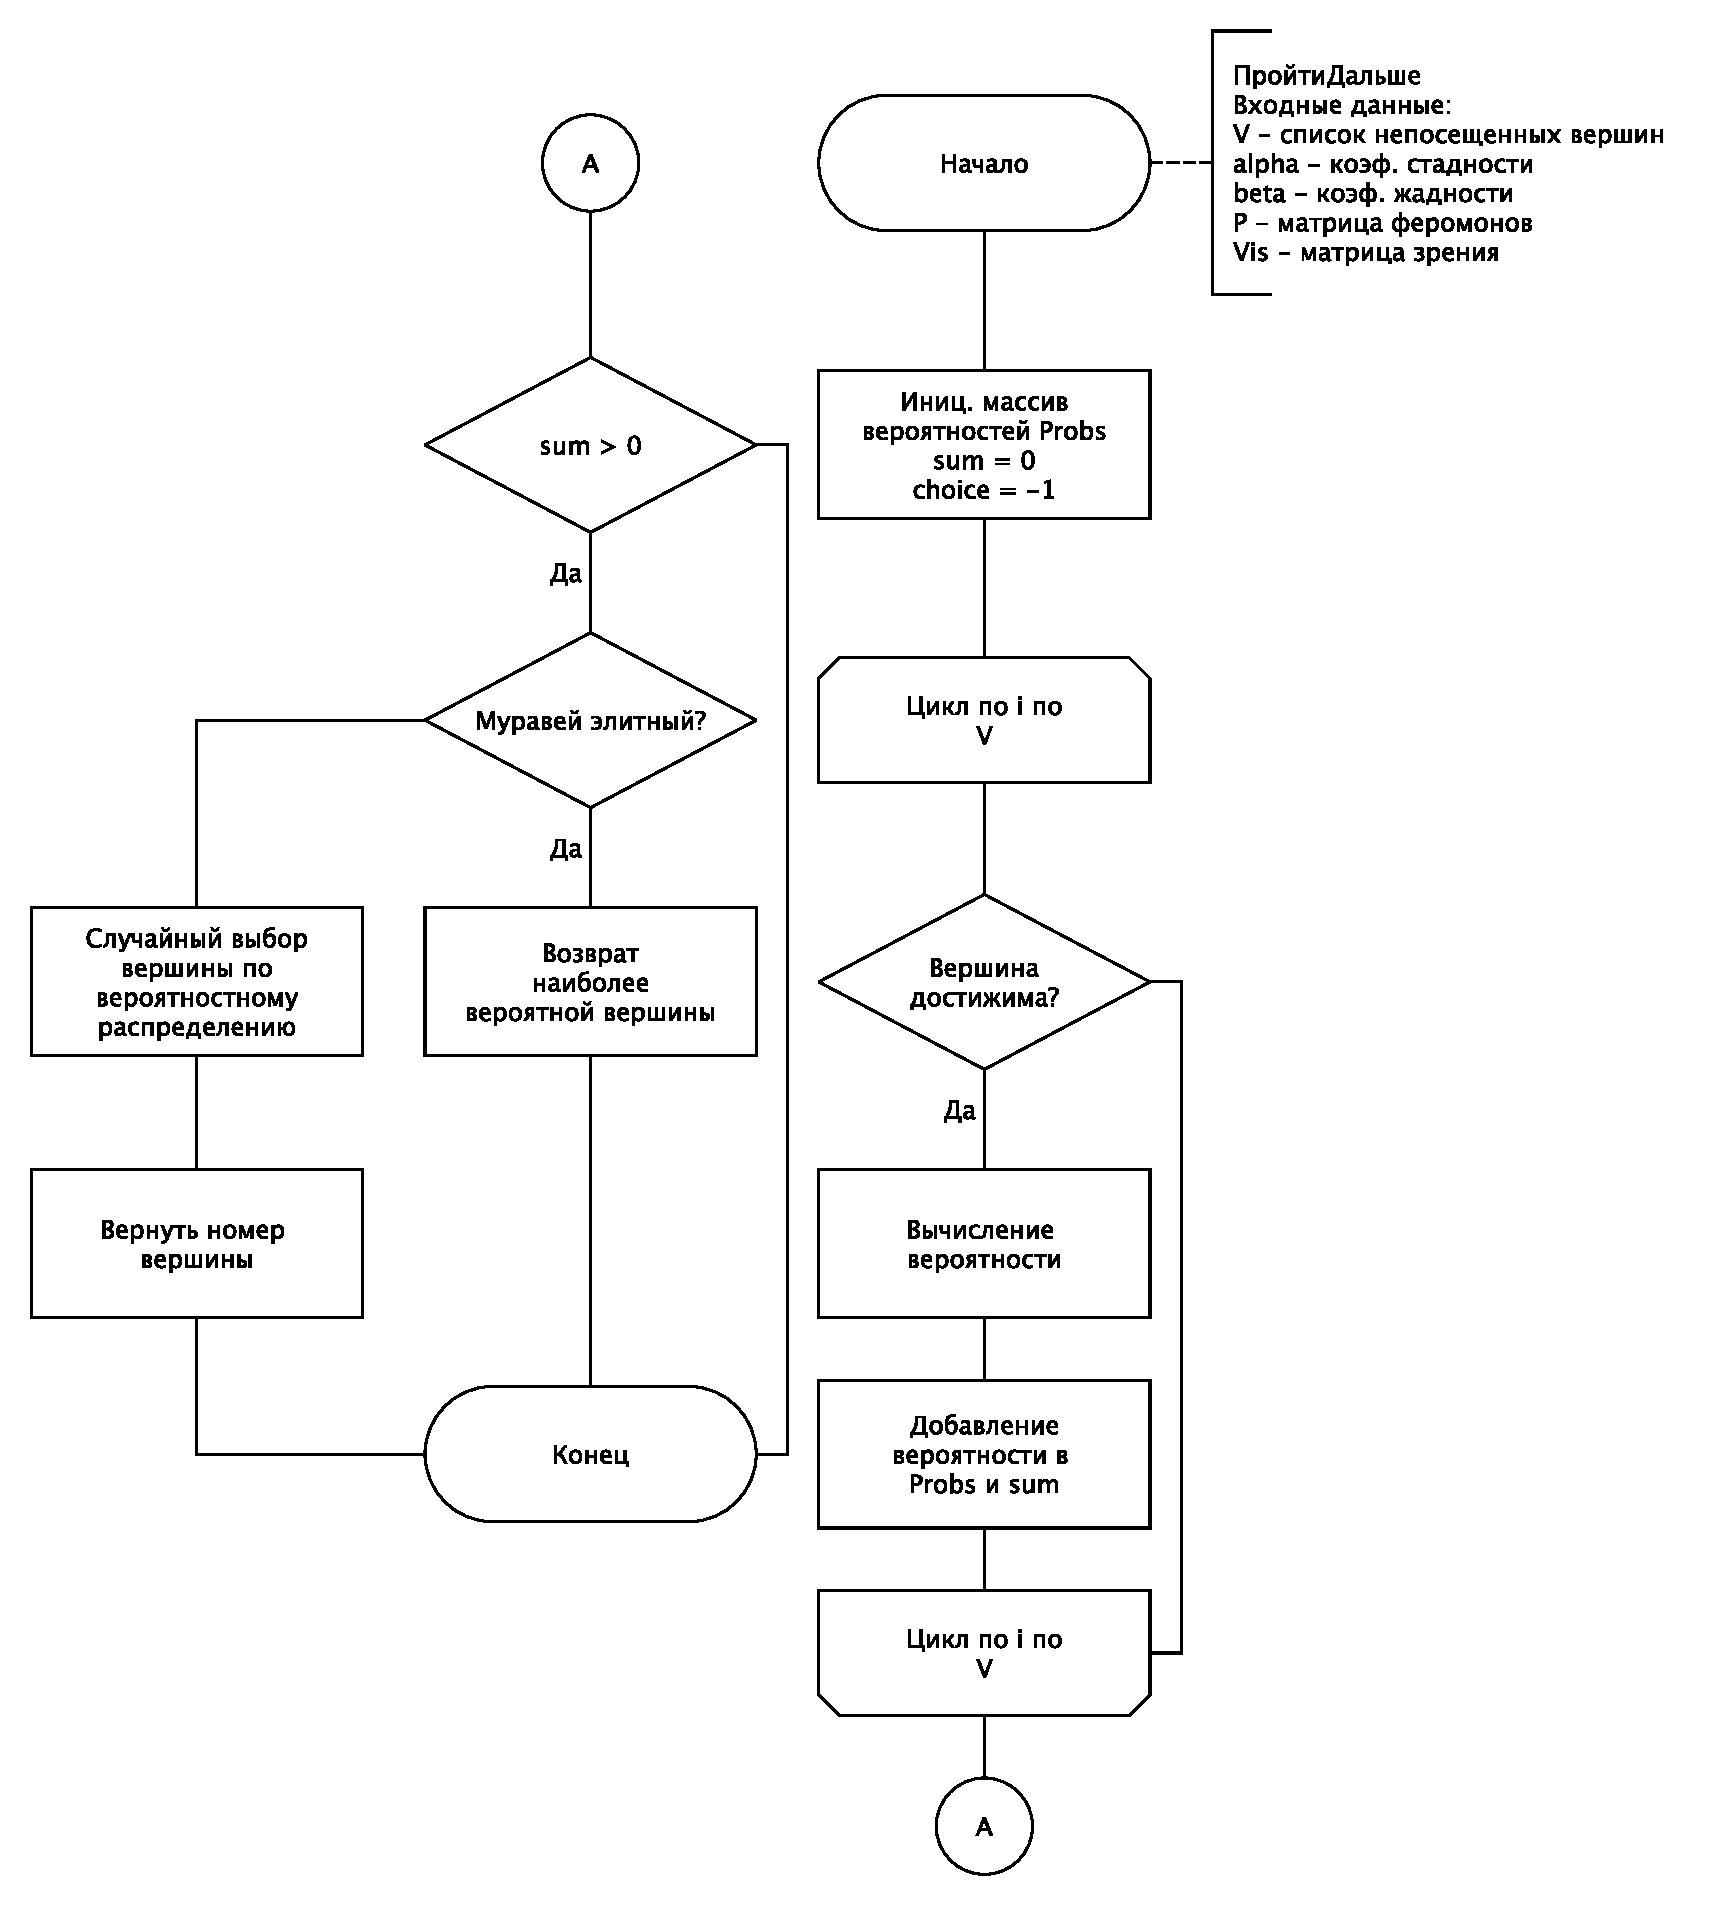
\includegraphics[width=0.9\linewidth]{schema2.pdf}
    \caption{Схема алгоритма перехода для одного муравья}
    \label{img:schema2}	
\end{figure}

\newpage

\begin{figure}[h!]
\centering
    \includegraphics[width=0.8\linewidth]{schema3.pdf}
    \caption{Схема алгоритма нахождения маршрута для одного муравья}
    \label{img:schema3}	
\end{figure}

\newpage

\begin{figure}[h!]
\centering
    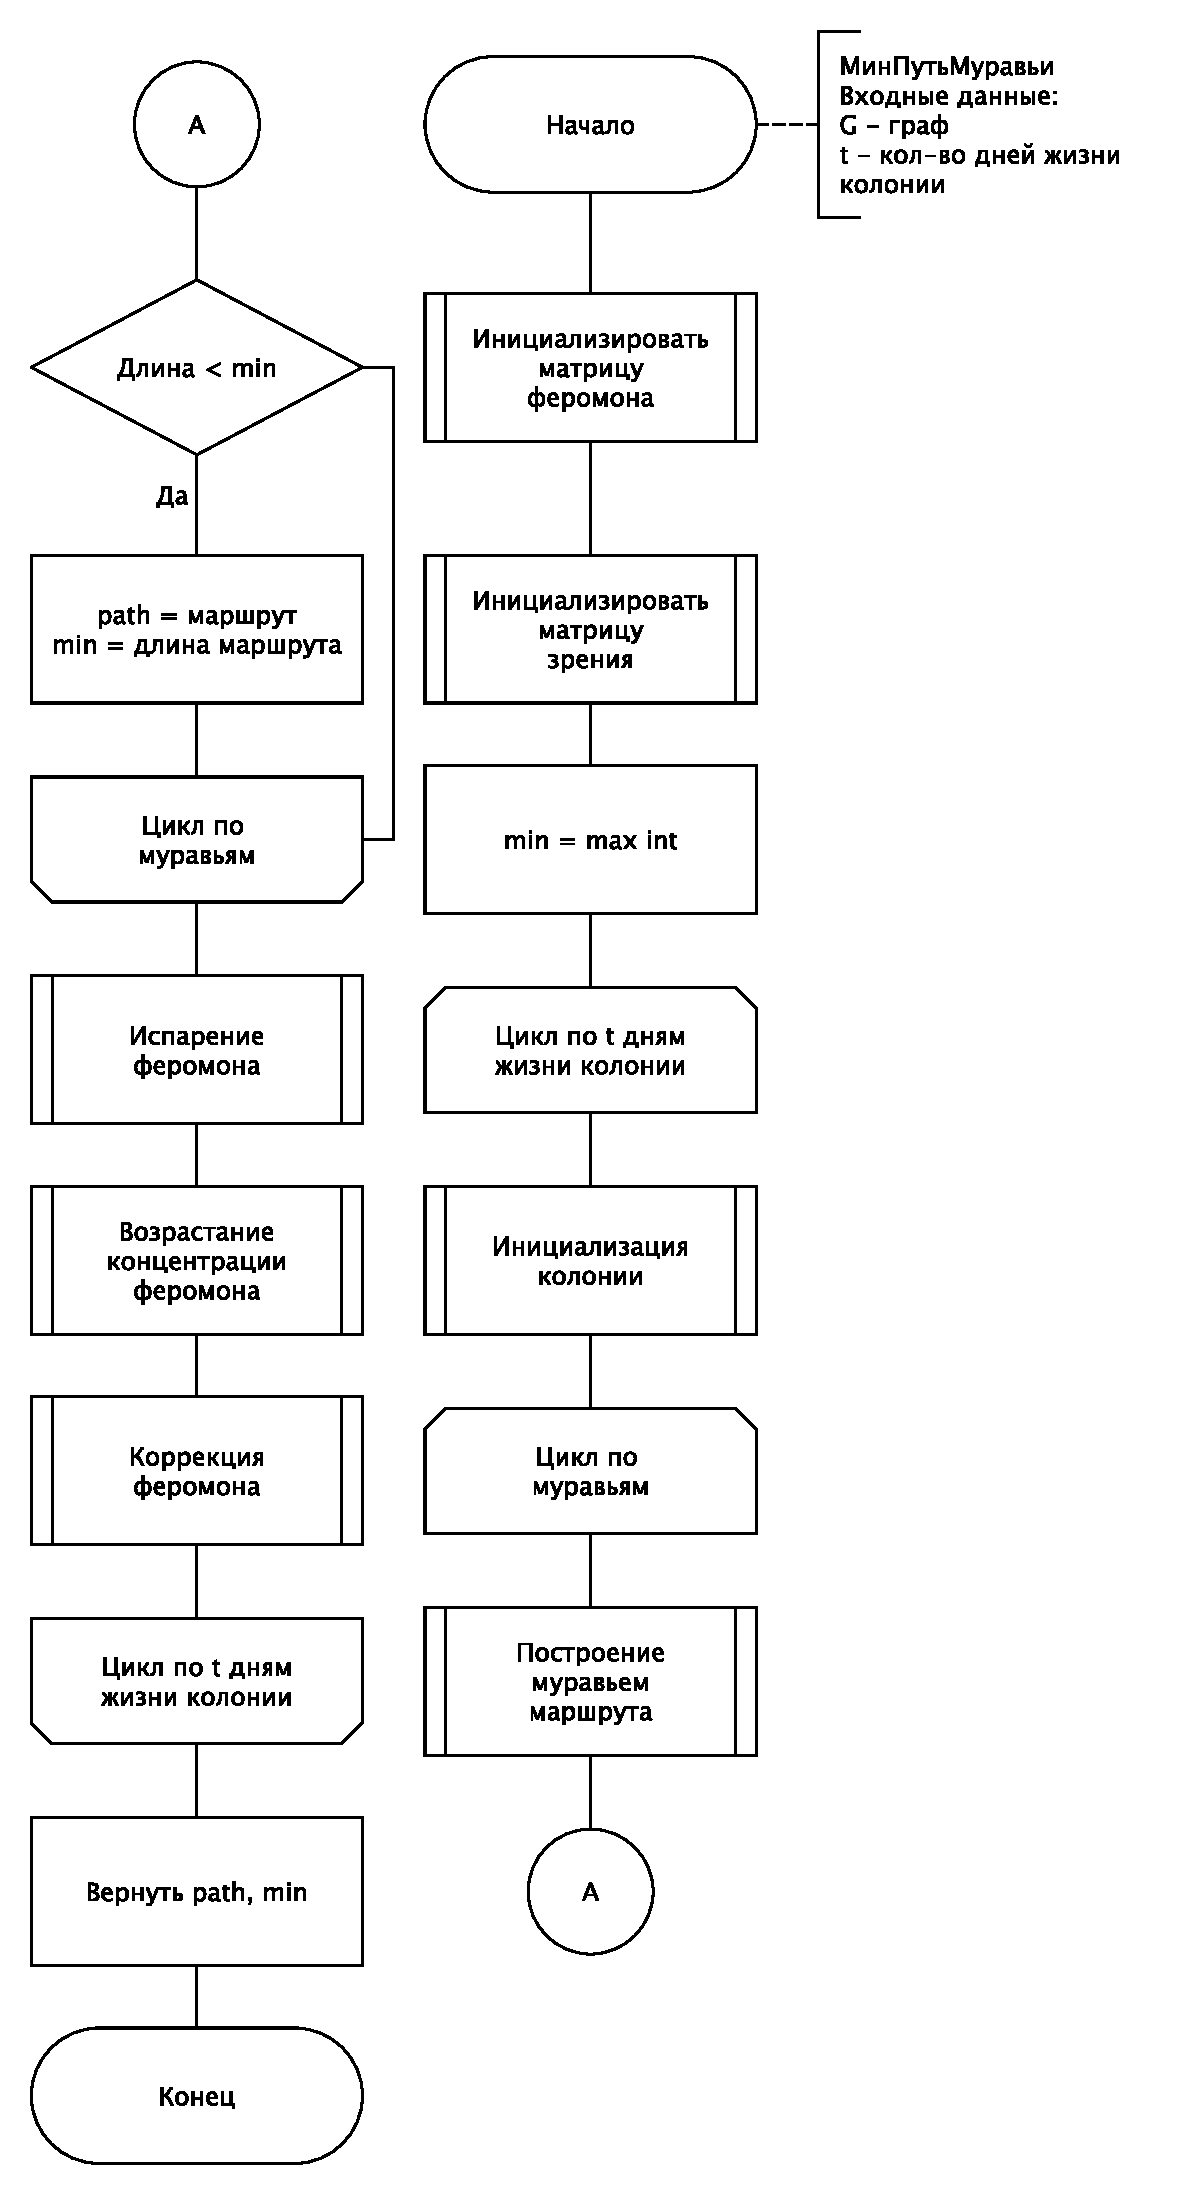
\includegraphics[width=0.6\linewidth]{schema4.pdf}
    \caption{Схема муравьиного алгоритма}
    \label{img:schema4}	
\end{figure}

\newpage

\section{Оценка трудоемкости алгоритмов сортировки}

\subsection{Модель вычислений}
Для вычисления трудоемкости исследуемых алгоритмов необходимо ввести модель вычислений. 

Если обозначить трудоемкость некоторой операции $a$, как $f_a$, то можно ввести таблицу соответствия значения трудоемкости для базовых операций:


\begin{table}[h]
  \caption{\label{table:complexity} Таблица значений тредоемкости}
  \begin{center}
    \begin{tabular}{|l|r|}
      \hline
      Операция & Трудоемкость\\ \hline
      $:=$ & $1$ \\ \hline
      $+=$ & $1$ \\ \hline
      $-=$ & $1$ \\ \hline
      $+$ & $1$ \\ \hline
      $-$ & $1$ \\ \hline
      $<<$ & $1$ \\ \hline
      $>>$ & $1$ \\ \hline
      $[]$ & $1$ \\ \hline
      $++$ & $1$ \\ \hline
      $--$ & $1$ \\ \hline
      $>=$ & $1$ \\ \hline
      $<=$ & $1$ \\ \hline
      $==$ & $1$ \\ \hline
      $!=$ & $1$ \\ \hline
      $<$ & $1$ \\ \hline
      $>$ & $1$ \\ \hline
      $*$ & $2$ \\ \hline
      $/$ & $2$ \\ \hline
      $\%$ & $2$ \\ \hline
      вызов функции & $0$ \\ \hline
    \end{tabular}
  \end{center}
\end{table}

Трудоемкость условного блока можно ввести следующим образом:

\begin{equation}
	f_{if} = f_{cond} + \begin{cases}
		min(f_{in\_if}, f_{in\_else}) \quad \text{в лучшем случае}, \\
		max(f_{in\_if}, f_{in\_else}) \quad \text{в худшем случае},
	\end{cases}
\end{equation}

где

\begin{itemize}
	\item $f_{if}$~---~трудоемкость условного блока;
	\item $f_{cond}$~---~трудоемкость вычисления условия;
	\item $f_{in\_if}$~---~трудоемкость фрагмента после $if$;
	\item $f_{in\_else}$~---~трудоемкость фрагмента после $else$.
\end{itemize}

Трудоемкость цикла можно ввести следующим образом:


\begin{equation}
	f_{loop} = f_{init} + f_{cmp} + n \cdot (f_{body} + f_{cmp} + f_{inc}),
\end{equation}

где

\begin{itemize}
	\item $f_{loop}$~---~трудоемкость цикла;
	\item $f_{init}$~---~трудоемкость инициализирующего выражения;
	\item $f_{cmp}$~---~трудоемкость сравнения цикла;
	\item $f_{body}$~---~трудоемкость тела цикла;
	\item $f_{inc}$~---~трудоемкость инкремента.
\end{itemize}

\subsection{Трудоемкость алгоритма полного перебора}

Здесь и далее, $N$~---~количество вершин графа.

Трудоемкость тела цикла равна

\begin{equation}
	f_1 = 2 + N \cdot 10 + 1 + 2 + N \cdot 12 = 5 + 22 \cdot N.
\end{equation}

Трудоемкость внешнего цикла равна
\begin{equation}
	f_2 = 2 + N! \cdot (2 + f_1) = 2 + N! \cdot (7 + 22 \cdot N).
\end{equation}

Трудоемкость алгоритма полного перебора равна трудоемкости внешнего цикла, поэтому

\begin{equation}
	f = f_2 = 2 + N! \cdot (7 + 22 \cdot N).
\end{equation}

Таким образом, асимптотику алгоритма полного перебора можно оценить как $O(N!)$.

\section{Трудоёмкость муравьиного алгоритма}
Пусть $T$~---~количество циклов жизни колонии.

Трудоемкость инициализации матрицы видимости равна
\begin{equation}
	f_1 = 1 + 2 + N \cdot 5 + 2 + N \cdot (2 + 2 + N \cdot 5) = 5 + 7 \cdot N + 5 \cdot N^2.
\end{equation}

Трудоемкость инициализации коэффициента пропорциональности феромона равна
\begin{equation}
	f_2 = 1 + 2 + N \cdot (2 + 2 + N \cdot 5) + 1 = 4 + 4 \cdot N + 5 \cdot N^2.
\end{equation}

Трудоёмкость инициализации матрицы феромонов равна
\begin{equation}
	f_3 = 1 + 2 + N \cdot 5 + 2 + N \cdot (2 + 2 + N \cdot 5) = 5 + 7 \cdot N + 5 \cdot N^2.
\end{equation}

Трудоемкость поиска муравьем следующей вершины для $n$ непосещенных вершин для элитных муравьев равна
\begin{equation}
	f_4 = 4 + (n - 1) \cdot 17 + 5 + (n - 1) \cdot 5 + 1 = -12 + 22 \cdot n.
\end{equation}

Трудоемкость поиска муравьем следующей вершины для $n$ непосещенных вершин для обычных муравьев равна
\begin{equation}
	f_4 = 4 + (n - 1) \cdot 17 + 5 + (n - 1) \cdot 8 + 7 + 4 \cdot n + 2 = -7 + 29 \cdot n.
\end{equation}

Трудоемкость поиска муравьем маршрута равна
\begin{equation}
	f_5 = 3 + N \cdot 4 + 1 + \sum{f_4} + N \cdot (10 + N \cdot 11) + 3.
\end{equation}

\begin{equation}
	f_5 = 5 - 9 \cdot N + 22 \cdot N^2.
\end{equation}

Трудоемкость создания колонии равна
\begin{equation}
	f_6 = 1 + 2 + N \cdot (2 + 7) = 3 + 9 \cdot N.
\end{equation}

Трудоемкость испарения феромона равна
\begin{equation}
	f_7 = 2 + N \cdot (2 + 2 + N \cdot (2 + 7)) = 2 + 4 \cdot N + 9 \cdot N^2.
\end{equation}

Трудоемкость прироста феромона равна
\begin{equation}
	f_{8} = 2 + N \cdot (2 + 2 + (N - 1) \cdot (2 + 9)) = 2 - 7 \cdot N + 11 \cdot N^2.
\end{equation}

Трудоемкость коррекции феромона равна
\begin{equation}
	f_{9} = 2 + N \cdot (2 + 2 + N \cdot 3) = 2 + 4 \cdot N + 3 \cdot N^2.
\end{equation}

Трудоемкость цикла по количеству муравьев в колонии равна
\begin{equation}
	f_{10} = 2 + N \cdot (2 + f_5 + 8) = 2 + 15 \cdot N - 9 \cdot N^2 + 22 \cdot N^3.
\end{equation}

Трудоемкость цикла по дням равна
\begin{equation}
	f_{11} = 2 + T \cdot (f_{6} + f_{10} + f_{7} + f_{8} + f_{9}),
\end{equation}

\begin{equation}
	f_{11} = 2 + 11 \cdot T + 25 \cdot N \cdot T + 14 \cdot N^2 \cdot T + 22 \cdot N^3 \cdot T.
\end{equation}


Трудоемкость муравьиного алгоритма равна
\begin{equation} 
	f = f_{1} + f_{2} + f_{3} + 2 + f_{11} + 5,
\end{equation}

\begin{equation} 
	f = 23 + 18 \cdot N + 15 \cdot N^2 + 11 \cdot T + 25 \cdot N \cdot T + 14 \cdot N^2 \cdot T + 22 \cdot N^3 \cdot T.
\end{equation}

Таким образом, асимптотика муравьиного алгоритма равна $O(T \cdot N^3)$.

\newpage